\documentclass[a4paper,12pt]{thesis}

\usepackage[utf8]{inputenc}

\usepackage{blindtext}


\usepackage[onehalfspacing]{setspace}

\usepackage{adjustbox}
\usepackage[ngerman]{babel}
\usepackage[T1]{fontenc}
\usepackage{amsfonts}
\usepackage{amsmath}
\usepackage{mathtools} 
\usepackage{mathabx}
\usepackage{graphicx}
\usepackage[table]{xcolor}
\usepackage{longtable}
%\usepackage{hyperref}

\usepackage{setspace}

\usepackage{color}
\usepackage{transparent}

\usepackage{tikz}
\usetikzlibrary{positioning}
\usetikzlibrary{arrows,calc}
%\usepackage{pgfplots} % LaTeX
\usepackage{colortbl}
%\usepackage{pgfplotstable}
\usepackage{booktabs, colortbl}

\usepackage{eurosym}

\usepackage{csvsimple}

\usepackage[authoryear]{natbib}
%\bibliographystyle{apalike}
\usepackage[hidelinks]{hyperref}
\bibliographystyle{apalike}

\newcommand*{\captionsource}[2]{%
	\caption[{#1}]{%
		#1%
		\\\hspace{\linewidth}%
		\textbf{Quelle:} #2%
	}%
}

\tikzset{
%Define standard arrow tip
>=stealth',
%Define style for different line styles
help lines/.style={dashed, thick},
axis/.style={<->},
important line/.style={thick},
connection/.style={thick, dotted},
}


\begin{document}

%%% TITELSEITE %%%

\begin{center}								% Beginn einer center-Umgebung. Der Text innerhalb der center-Umgebung wird zentriert. Ansonsten wird Blocksatz verwendet
	\begin{LARGE}								% LARGE beschreibt eine Schriftgröße in Latex. Der Standard ist \normalsize. Eine übersicht der Schriftgrößen steht z.B. auf der Seite: https://www.latex-kurs.de/fragen/schriftgroesse.html 
		Faktoren des Fahrrad Verkehrs in Mannheim						% Text, der nun zentriert und in größerer Schrift geschrieben wird 
	\end{LARGE}								% Die Verwendung der Schriftgröße LARGE wird beendet. Es gilt ab jetzt wieder die normale Schriftgröße.
	
	\vspace{\fill}								% Befehl, der den vertikalen Platz (vspace) "füllt" 
	
	\begin{large}								% Der folgende Text hat nun die Schriftgröße large 
		Maximilian Samuel Weinhold\\					% Durch ein \\ wird eine neue Zeile angefangen. 
		Economics, 6. Semester\\
		505314\\
		mweinhol@uni-muenster.de\\
		
		\vspace{\fill}
		
		Hausarbeit im Rahmen des Seminars zur\\
		Analyse von Fahrrad-Verkehrsdaten\\
		Sommersemester 2021\\
		Institut für Verkehrswissenschaft\\
		Dr. Jan Wessel\\
	\end{large}
	
	\thispagestyle{empty}						% Definiert den Stil für diese Seite. empty bedeutet, dass keine Seitenzahl auf der Seite gedruckt wird. 
	
\end{center}								% Ab nun wird wieder Blocksatz verwendet

\newpage									% Seitenumbruch. Es beginnt eine neue Seite


%\chapter*{Tabellen und Abbildungen}\addchapmark{Tabellen und Abbildungen}
\onehalfspacing	
\thispagestyle{empty}	
\tableofcontents
%\begingroup
%\let\clearpage\relax
%\listoffigures
%\endgroup

%\newpage

%\listoffigures

%\newpage


%\listoffigures
%\addcontentsline{toc}{chapter}{Abbildungsverzeichnis}

\chapter{Einleitung}

Die mobile Infrastruktur urbaner Zentren in Deutschland unterliegt einem Wandel, der nicht mehr allein das Ziel einer autofreundlicheren Stadt hat, sondern auch andere Verkehrsteilnehmer hervor hebt. Im besonderen betrifft diese Entwicklung auch das Fahrrad. So ist laut \cite{Nobis2019} die Anzahl der Fahrradfahrer und die von ihnen zurückgelegten Wege innerhalb von 15 Jahren stark angestiegen und ebenso der Ausbau von Fahrradwegen. Ein Beispiel für diese Entwicklungen ist Mannheim. Denn hier verfolgt die städtische Planung ein 21 Punkte Programm, dass dazu dienen soll den Anteil des Radverkehrs zu steigern.\\
Im Rahmen dieses Programms installierte die Stadt an verschiedenen Stellen 8 Fahrradzähler, deren stündlichen Zählungen öffentlich abrufbar sind. Mithilfe dieser Daten wollen wir versuchen ein Model zu entwickeln, dass die kausal Einflüsse auf den Radverkehr erklärt und das Aufkommen von Fahrrädern vorhersagen kann. Im besten Fall extrapolieren wir das Model und prüfen, ob wir das Model auch auf Bereiche außerhalb der Zählstellen anwenden können.\\
Bei diesem Vorhaben bauen wir vornehmlich auf \cite{Wessel2020}, der primär untersuchte welchen Einfluss Wettervorhersagen und tatsächliches Wetter auf den Radverkehr in verschiedenen deutschen Städten hat. Dazu nutzen wir Daten des Deutschen Wetter Dienstes.\\
Darüber hinaus (Wenn Zeit übrig bleibt) wollen wir versuchen die Methoden von \cite{PRATI201744} ebenfalls zu verwenden, um ein Model primär zu Vorhersage des extrapolierten Fahrradaufkommens zu entwickeln.

\chapter{Literaturüberblick}

Da diese Arbeit im Rahmen eines Seminares bei Dr. Jan Wessel entstanden ist, verfolgt diese Arbeit eine ähnliche Methodik wie bei \cite{Wessel2020}, der der Frage nachgeht, wie sehr Wettervorhersagen und tatsächliches Wetter einen Einfluss auf das Aufkommen der Fahrradfahrer hat. Dazu entwickelt er ein log-lineares Regressionsmodel, das nicht nur die notwendigen Wetterdaten berücksichtigt, sondern auch andere wesentliche Effekte, wie Feiertage, Schul- und Semesterferien. Sein Model kommt zu einem adjusted $R^2$ von 78 \%. Die Daten für das Model stammen von 188 Zählstationen in ganz Deutschland.\\

Hier noch mehr bearbeiten. Vor allem im Bezug auf die eigene Vorschungsfrage.

\chapter{Beschreibung der Daten}

Zur Bearbeitung des Models nutzen wir vornehmlich zwei Daten Quellen. Zum einem nutzen wir die Daten der Fahrradzählstationen Mannheims, die öffentlich im Netz zugänglich sind (Link: https://mannheim.opendatasoft. com/page/home/). Hier sind stündliche Werte gezählter Fahrräder verfügbar an 8 verschiedenen Stellen in der Stadt, sowie Längen und Breitengrad der Position, Standortname, Zeit und Datum. Diese Daten verbinden wir mit stündlichen Daten des Deutschen Wetter Dienstes zur Lufttemperatur in 2 Meter Höhe, zur relativen Feuchte, zum Bedeckungsgrad, zum Niederschlag und zur Sonnenstrahlung.\\
\cite{ZHAO2018826} und \cite{Hong2022} zeigen, dass auch Feinstaubbelastung den Radverkehr beeinflussen kann. Und grundsätzlich wären die dazu notwendigen Daten aus Mannheim über Opensensemap.org auch zugänglich, jedoch nicht welche, die weit genug zurückreichen, um den gesamten Betrachtungszeitraum zu beachten. Da \cite{ZHAO2018826} und \cite{Hong2022} ihre Forschung in Ostasiatischen Ballungsräumen betrieben haben und in einer Stadt wie Mannheim nicht die selbe Feinstaubbelastung zu erwarten ist, kann man von dieser Variable nicht erhoffen, dass sie die notwendige Erklärungskraft bringt, um einen Wegfall des Betrachtungszeitraumes zu rechtfertigen, weshalb Feinstaubmessungen keinen Weg in den Datensatz gefunden haben.\\
Dafür ist es wichtig Feiertage, Schulferien und Semesterferien zu berücksichtigen. Hier könnte potentiell eine geographische Besonderheit Mannheims eine Rolle spielen, denn das Stadgebiet grenzt direkt zu zwei verschiedenen Bundesländern an. Zum einem liegt auf dem gegenüberliegenden Rheinufer die Stadt Ludwigshafen, die bereits in Rheinland Pfalz liegt. Zwischen beiden Städten herrscht ein reger Verkehr, weshalb anzunehmen ist, dass voneinander abweichende Feiertage in Rheinland Pfalz und Badenwürttemberg eine Rolle spielen könnten. Ebenso grenzt Hessen an Mannheim an. Jedoch nicht in einer Reichweite, die für Fahrradfahrer realistisch erscheint und nicht mit einer Stadt, die vergleichbar grroß wie Ludwigshafen wäre. Somit finden Feiertage für Hessen keinen Weg ins Model.\\
Dies gilt ebenso für die Schulferien. Es ist anzunehmen, dass innerhalb Mannheims, Schulen von Mannheimern überwiegend besucht werden, weshalb nur die Schulferien von Baden Württemberg im Datensatz zu finden sind. Neben Schülern fahren ebenso häufig Studenten Fahrrad als günstigstes Verkehrsmittel. Die größte Hochschulbildungseinrichtung ist die Universität Mannheim, deren Semeseterferien eine signifikante Rolle spielen dürften.

\begin{figure}[!ht]
	\centering
	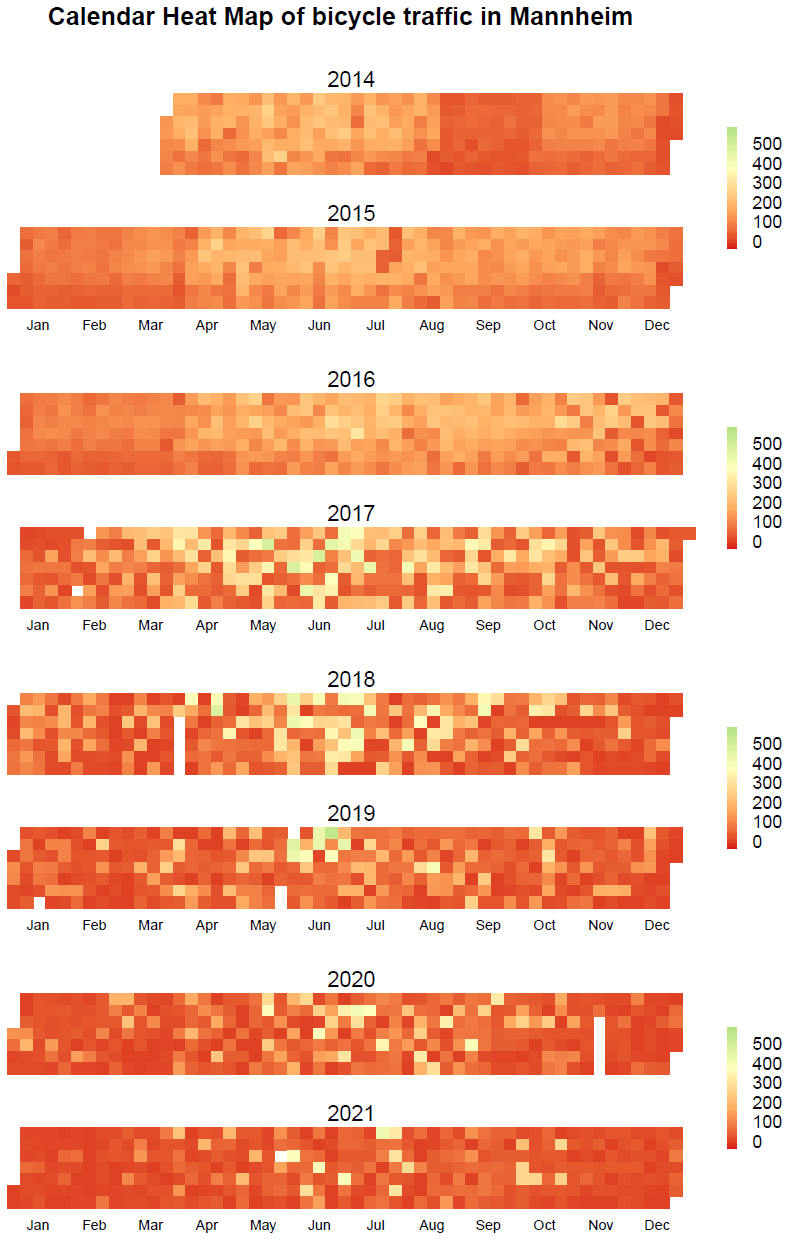
\includegraphics[width=\textwidth]{Plots/CalendarHeatMap.png}
	\captionsource{Heat Map}{
		Ausprägungen des Fahrradaufkommens
	}
	\label{fig:calendarheatmap}
\end{figure}

Fügt man all diese Daten zusammen, erhält man einen Datensatz der 410891 Beobachtungen umfasst. Die Ausprägungen pro Tag sind der Darstellung \ref{fig:calendarheatmap} zu entnehmen. Dabei fallen zwei Dinge vornehmlich auf. Zum einem sehen wir, wie gegen Ende 2016 die Varianz der Ausprägungen zu nimmt. Dies hängt mit der Anzahl der Zählstationen zusammen. Die früheste Zählstation an der Renzstraße ging 2014 in Betrieb. Weiter folgten erst 2016. Je mehr Zählstationen mit unterschiedlichen Verkehrsströmen messen, desto höher ist die tägliche Varianz in den Zähldaten. Weiterhin fallen einige wenige weiße Stellen auf. Dies hängt mit unvollständigen Wetterdaten zusammen. Die Menge fehlender Daten fällt hier aber in einen vertretbaren Rahmen, wobei fehlende Tage nicht weiter mit wichtigen Variabeln korrelieren.

\section{EcoCounter Mannheim}

In Mannheim gibt es 8 verschiedene Stationen. Einen Überblick über diese Stationen ist in Abbildung X zu sehen, wobei zu Erstellung der Graphik ein R Paket genutzt wurde nach \cite{Kahle2013}. Am Farbgradienten ist zu sehen, wie viele Fahrradfahrer pro Stunde die Zählstationen passieren. Zudem ist der Name der Zählstation eingeblendet zudem das Jahr, seitdem diese Zählstation installiert ist. Die älteste Station hier ist die Renzstraße. Jedoch zählte diese während einer Unterbrechung vom ... bis ... nicht.\\
Weiter Variablen wurden aus den Datumsvariabeln erzeugt. So haben wir eine Dummy Variable für Wochenende eingefügt und eine für Sommermonate. Weiterhin nutzen wir Jahr, Monat, Tag und Stunde als Faktorvariablen, wobei wir nächtliche Stunden zwischen 22 und 5 Uhr ausgeschlossen haben.\\
Zu Abweichungen des Fahrradverkehrs konnte es während Corona kommen, wo Teile des öffentlichen Lebens still standen und damit auch das Verkehrsaufkommen. Deshalb haben wir drei Variablen in das Modell aufgenommen.

\begin{figure}[!ht]
	\centering
	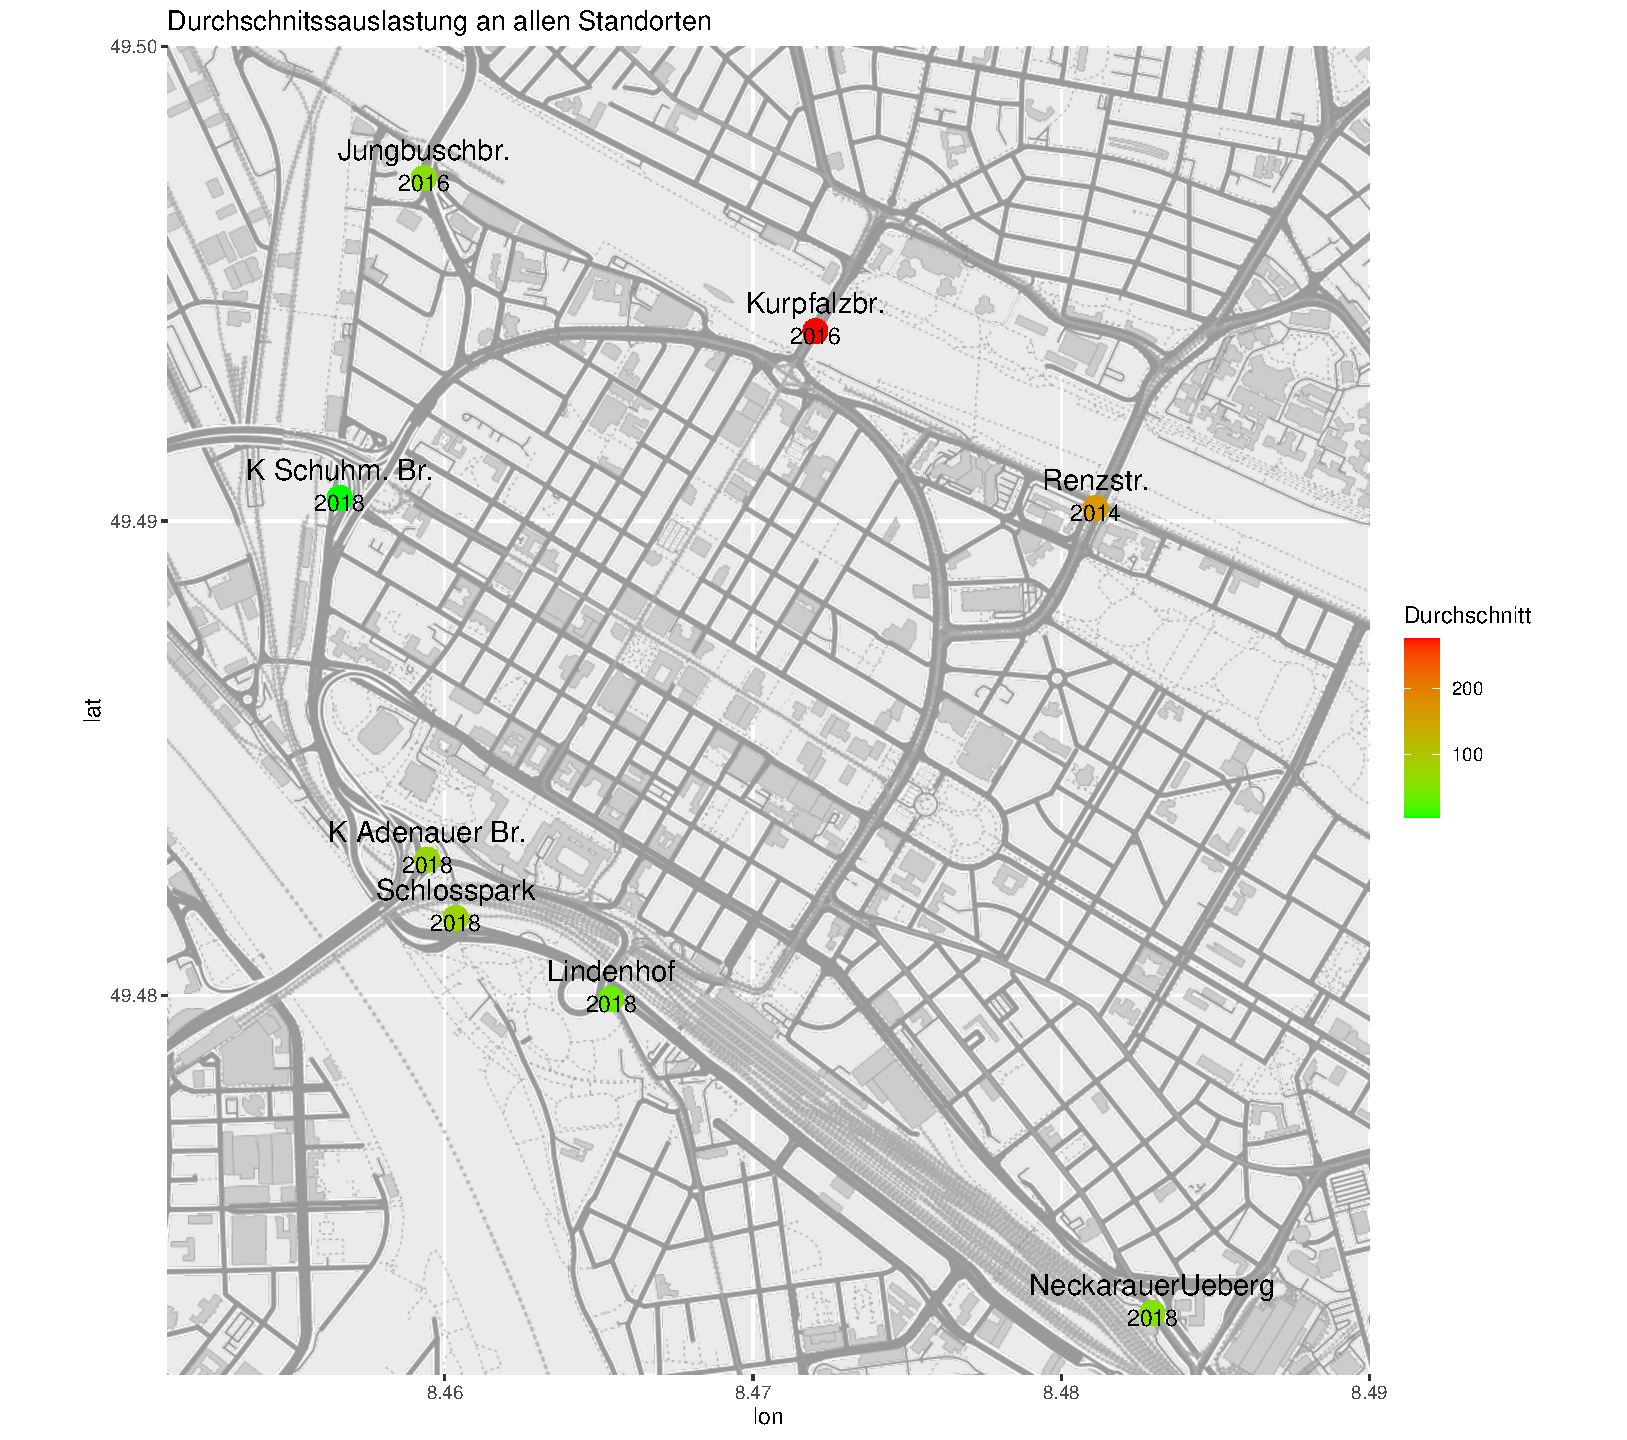
\includegraphics[width=\textwidth]{Plots/Karte_Durchschnittsauslastung.pdf}
	\captionsource{Zählstationsüberblick Mannheim}{
		Zählstation nach Durchschnitt pro Stunde und Startjahr
	}
	\label{fig:meine-grafik5}
\end{figure}



\begin{figure}[!ht]
	\centering
	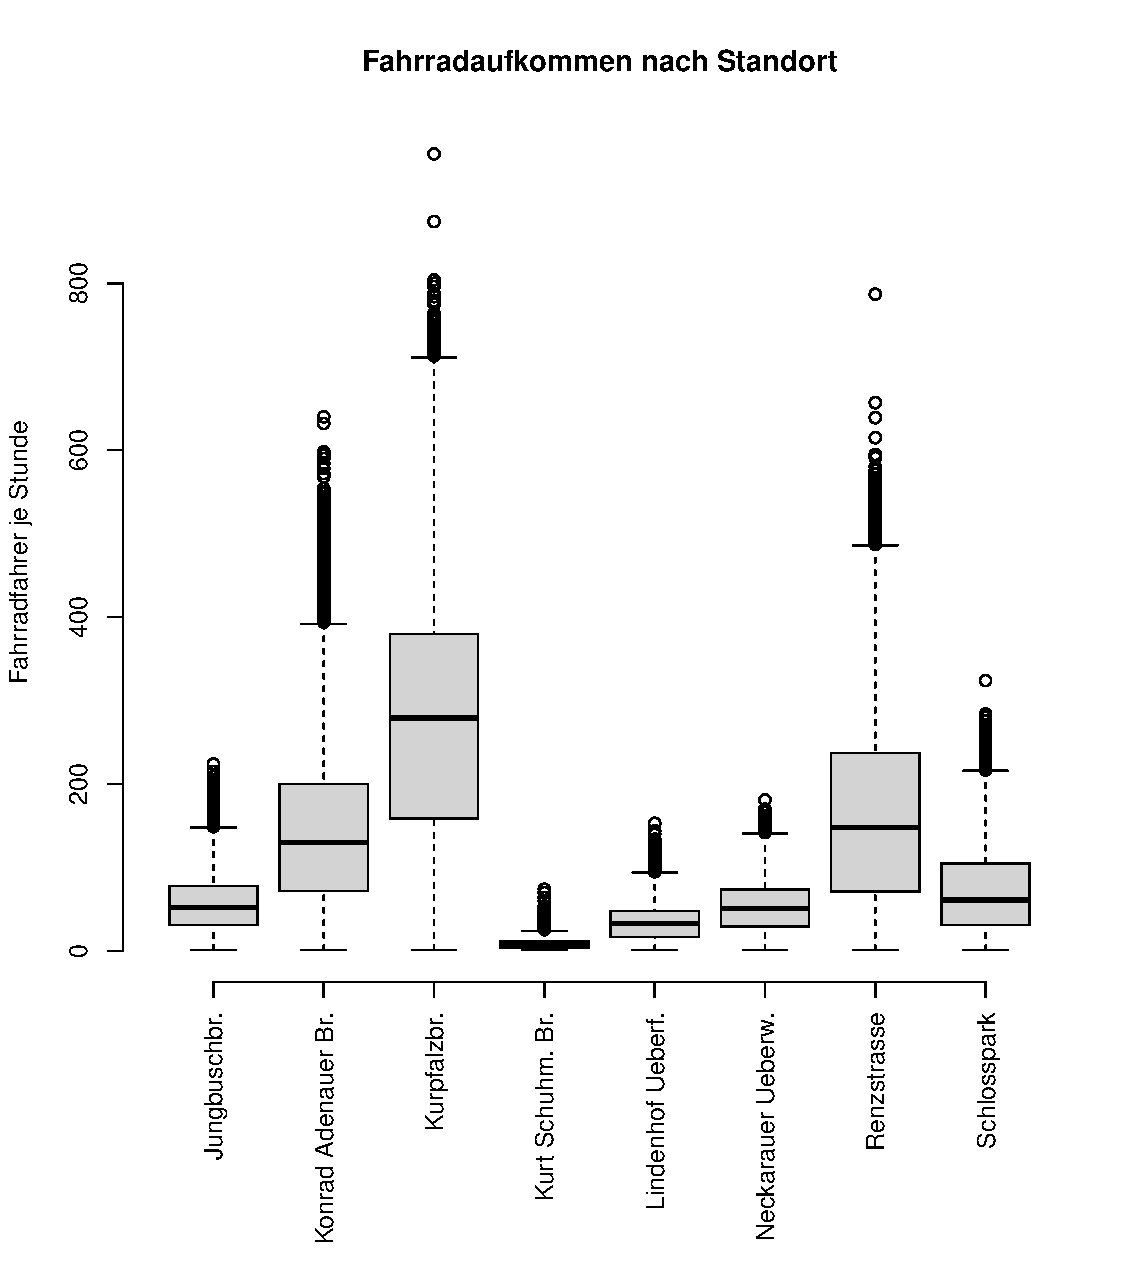
\includegraphics[width=\textwidth]{Plots/Boxplot_Stationen.pdf}
	\captionsource{Boxplots zu den Zählstationen}{
		Verteilung der Fahrräder pro Stunde
	}
	\label{BoxplotStationen}
\end{figure}

\section{DWD Daten}

\begin{table}[!ht]
	\centering
	\begin{tabular}{rllllll}
		\hline
		Name & Min & Durchschnitt & Max & Stand.abw. & Korrelation \\ 
		\hline
		Zaehlstand & 1 & 108.35 & 955 & 120.21 & 1 \\ 
		Distanz z Uni & 208.36 & 1122.51 & 1875.72 & 583.35 & 0.26 \\ 
		Wochenende & 0 & 0.28 & 1 & 0.45 & -0.21 \\ 
		Sommer & 0 & 0.48 & 1 & 0.5 & 0.15 \\ 
		Feiertag BW & 0 & 0.03 & 1 & 0.18 & -0.09 \\ 
		Feiertag RP & 0 & 0.03 & 1 & 0.18 & -0.08 \\ 
		Schulferien BW & 0 & 0.32 & 1 & 0.47 & 0.04 \\ 
		Semesterferien & 0 & 0.48 & 1 & 0.5 & -0.03 \\ 
		WertRR & 0 & 0.07 & 30.4 & 0.49 & -0.03 \\ 
		QualitaetRR & 3 & 3 & 3 & 0 &  \\ 
		WertT2M & -13 & 12.67 & 39.4 & 8.33 & 0.24 \\ 
		QualitaetT2M & 3 & 6.93 & 7 & 0.51 & 0.05 \\ 
		WertF & 0.1 & 3 & 14.4 & 1.65 & -0.02 \\ 
		QualitaetF & 3 & 9.67 & 10 & 1.16 & 0.1 \\ 
		WertRF & 14 & 69.24 & 100 & 20.3 & -0.23 \\ 
		QualitaetRF & 3 & 6.93 & 7 & 0.51 & 0.05 \\ 
		WertSD & 0 & 19.22 & 60 & 24.82 & 0.17 \\ 
		QualitaetSD & 3 & 9.33 & 10 & 1.42 & 0.1 \\ 
		WertN & 0 & 5.72 & 8 & 3.14 & -0.08 \\ 
		QualitaetN & 3 & 3 & 3 & 0 &  \\ 
		Corona & 0 & 0.42 & 1 & 0.49 & -0.16 \\ 
		Kontaktbeschr & 0 & 0.11 & 1 & 0.32 & -0.09 \\ 
		TagesAusbr & 0 & 143.48 & 687 & 212.5 & -0.17 \\ 
		\hline
	\end{tabular}
	\label{Tabelle1}
\end{table}

Notiz für später: Am besten wertest du die Qualitätsdaten genauer aus.

\chapter{Deskriptive Analyse}




\section{Regressionsanalyse}

Vorerst sind die gesammelten Daten trotz des Umfang recht nutzlos, da sie allein wenig Antworten geben. Durchschnitte und Standardabweichungen einzelner Variablen wie der Temperatur oder des Fahrrad Aufkommens, gäben durchaus Aufschluss nie aber in einem größeren Zusammenhang. Was wir vornehmlich in Erfahrung bringen möchten ist, was den Fahrradverkehr beeinflusst. Dies mündet z.B. in der Frage welchen Einfluss der Regenfall auf den Fahrradverkehr ausübt, oder ob mehr Fahrradfahrer an Feiertagen auf Mannheims Straßen anzufinden sind. Dies wollen wir nicht nur qualitativ beantworten, sondern auch quantitativ.\\

Ein Mittel um an diese Informationen zu kommen ist die Regressionsanalyse. Diese versucht den Zusammenhang zu messen, in dem zwei Variablen zu einander stehen. So könnte man zb versuchen zu messen, wie sehr die Lufttemperatur in zwei Meter Höhe das Aufkommen von Fahrrädern in Mannheim beeinflusst, dargestellt in der Abbildung \ref{fig:BSP}. Mithilfe der Regressionsanalyse kann man nun durch diese in diesem Fall sehr dichte Punktwolke jene Linie ziehen, die das Verhältnis mathematisch am besten repräsentiert. Natürlich verhält sich nicht alles linear zu einander. In der Darstellung sieht man bereits, dass das Fahrradaufkommen bis knapp über 20 °C steigt, danach aber wieder rapide sinkt, das es den Leuten schlicht zu heiß wird. Dies kann manchmal mit einer nicht linearen Funktion dargestellt werden. Aber wie man sieht, egal ob man einen linearen, quadratischen oder kubischen Zusammenhang sieht, die eingezeichneten Regressionslinien erwecken nicht den Eindruck, den wahren Zusammenhang widerzuspiegeln, denn die beobachteten Werte also die eingezeichneten Punkte liegen weit auseinander. Das bedeutet der Fit unseres Models ist gering, allein mit der Außentemperatur können wir die Variation im Fahrradverkehr selbstverständlich nicht erklären.\\

\begin{figure}[!ht]
	\centering
	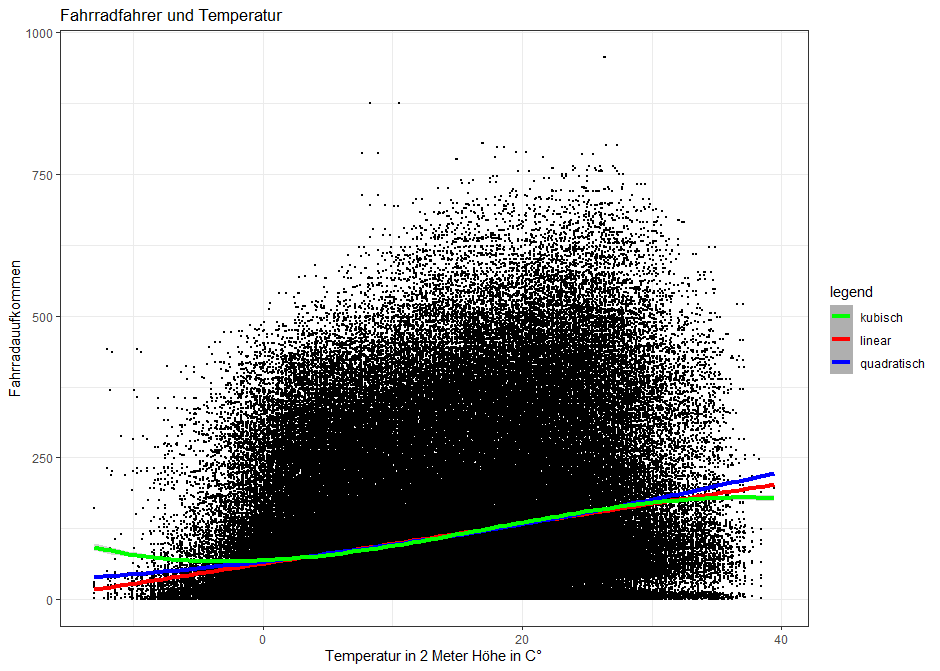
\includegraphics[width=\textwidth]{Plots/Regression_Bsp.png}
	\captionsource{Fahrrad Daten Mannheim und DWD}{
		Graphisches Beispiel einer Regression
	}
	\label{fig:BSP}
\end{figure}

Nehmen wir weitere Variablen in das Regressionsmodel auf, die den Fahrradverkehr erklären können, wie z.B. Wetterbeobachtungen oder Ferien- und Feiertage, dann steigt der Fit des Models. Das heißt wir können präzisere Vorhersagen treffen, weil wir uns ein mehrdimensionales Model schaffen. Dies nennt man dann auch die multiple Regressionsanalyse. Lässt man wiederum wichtige Variablen aus, dann kann das auch die Aussage über die Kausalität verzerren durch den Bias einer ausgelassenen Variable. Deswegen ist es wichtig, die richtigen und sinnigen Variablen in das Model aufzunehmen. Im folgenden Model haben sind nicht nur Wetterdaten und Ferien- Feiertage mit inbegriffen. Zusätzlich verwenden wir eine Dummy Variable für die Sommer Monate und eine Dummy Variable für alle Zeiträume, die von Corona Kontaktbeschränkungen betroffen waren. Nicht direkt dargestellt in der Übersicht \ref{reg1}, sind Dummy Variablen, für die vollen Stunden, Wochentage, Monate und Jahre, sowie der den Namen der Station als Faktor, damit das Modell zwischen den verschiedenen Leveln der Zählstationen unterscheiden können, denn der Verkehr an den einzelnen Stationen weicht stark voneinander ab, wie man in der Darstellung \ref{BoxplotStationen} sieht.\\

\begin{table}[!ht]
	\centering
	\caption{Log-Lineares Regressionsmodell}
	\begin{tabular}[t]{lc lc lc lc lc lc}
		\toprule
		& Koeffizient & Std Abw & t-Wert & Pr(>|t|) & \\
		\midrule
		%Intercept & -0.184 & (0.015) &\\
		Leichter Nieselregen & -0.184 & (0.015) & -12.12259 & 5.9389e-06 & ***\\
		Starker Nieselregen & -0.249 & (0.012) & -20.60850 & 1.5899e-07 & ***\\
		Leichter Regen & -0.331 & (0.021) & -15.84990 & 9.6482e-07 & ***\\
		Moderater Regen & -0.353 & (0.019) & -18.79747 & 2.9962e-07 & ***\\
		Starker Regen & -0.373 & (0.043) & -8.61747 & 5.6532e-05 & ***\\
		Heftiger Regen & -0.209 & (0.051) & -4.05542 & 4.8375e-03 & **\\
		Temperatur & 0.036 & (0.005) & 7.63981 & 1.2217e-04 & ***\\
		Temperatur$^2$ & -0.0005 & (0.000) & -9.29870 & 3.4479e-05 & ***\\
		Wind & -0.041 & (0.003) & -16.05586 & 8.8335e-07 & ***\\
		rel. Feuchte & -0.004 & (0.001) & -3.51258 & 9.8253e-03 & **\\
		Sonne & -0.0001 & (0.000) & -1.37325 & 2.1204e-01 & \\
		Bedeckung & -0.009 & (0.001) & -8.05733 & 8.7084e-05 & ***\\
		FeiertagBW & -0.460 & (0.081) & -5.69499 & 7.3917e-04 & ***\\
		FeiertagRP & -0.414 & (0.059) & -7.00091 & 2.1138e-04 & ***\\
		SchulferienBW & -0.139 & (0.020) & -6.84816 & 2.4239e-04 & ***\\
		SemesterferienUM & -0.159 & (0.031) & -5.19710 & 1.2570e-03 & **\\
		Sommer & 0.082 & (0.021) & 3.99890 & 5.1972e-03 & **\\
		Kontaktbeschr & -0.133 & (0.027) & -5.01609 & 1.5372e-03 & **\\
		\midrule
		Num.Obs. & 410891& & RMSE & 0.62 & \\
		R2 & 0.818& R2 Adj. & 0.818 &  & \\
		\bottomrule
		Fixed Effects & Standort & Stunde & Wochentag & Jahr & \\
		Note: & *p<0.1; & **p<0.05; &***p<0.01 & &\\
	\end{tabular}
\label{reg1}
\end{table}

Interessant sind für uns in der Darstellung \ref{reg1} die Koeffizienten und die Signifikanzniveaus. Wobei wir berücksichtigen müssen, dass wir ein Log-Lineares Modell verwendet haben. Das heißt wir haben die abhängige Variable den Zählstand der Fahrradstation logarithmiert, um nicht lineare Einflüsse modellieren zu können. Die Signifikanzniveaus werden durch Sterne gekeinzeichnet. Drei Sterne markieren das höchste Sighnifikanzniveau, kein Stern bedeutet, der kausalen Einfluss eines Koeffizienten ist statistisch signifikant, also zu klein im Verhältnis zur Streuung der Daten. Die Vorzeichen der Koeffizienten zeigen uns, ob eine Variable dazu führt, ob weniger Leute Fahrrad fahren, wenn zb. Regen fällt, oder weniger.\\ 
Den Regenfall haben wir kategorisiert, nach derselben Methode wie sie \cite{Wessel2020} verwendet. Auffällig ist, dass der heftige Regen wohl einen kleineren negativen Einfluss, als leichter Regen. Erklärbar wäre diese Beobachtung vielleicht dadurch, dass heftiger Regen oft plötzlich kommt und Fahrradfahrer überraschen kann. Auch der Mangel an Beobachtungen könnte dazu führen, denn heftiger Regen kommt selten vor, weshalb sein Signifikanzniveau auch geringer ist. Ansonsten sehen wir, dass zunehmender Regen einen zunehmend negativen Effekt hat. Für die Temperatur haben wir einen linearen und einen quadratischen Term in das Model aufgenommen, denn wie man in Darstellung \ref{fig:BSP} z.B. sieht, führen steigende Temperaturen nur solange zu mehr Fahrradverkehr, solange es nicht zu heiß wird. Die quadratische Funktion kann das gut repräsentieren. Allerdings sind alle anderen Wetterbeobachtung längst nicht so einflussreich wie der Regen. Die Sonneneinstrahlung ist sogar insignifikant.\\
Einen recht starken Einfluss haben die Feiertage. Wobei wir unterschieden haben in Feiertage in Baden Württemberg und Rheinland Pfalz. Hierbei sind die Effekte der Feiertage interessanterweise negativ. Dies gibt uns einen Hinweis darauf, dass in Mannheim ein utillitaristischer Fahrradverkehr vorherrscht. Also ein Fahrradverkehr, der nicht der eigenen Unterhaltung und Erholung dient, sondern um einen Zweck zu erfüllen. In den meisten Fällen wird es sich hierbei also um Berufsverkehr handeln bzw. Verkehr hin zu den Bildungsstätten der Stadt. Darauf weisen auch die negativen Effekte für die Schulferien in Baden Württemberg und die Semesterferien der Universität Mannheim hin. Schulferien für Rheinlandpfalz befinden sich nicht im Modell, weil ich angenommen habe, dass Schüler aus Ludwigshafen auch grundsätzlich in Ludwigshafen zur Schule gehen würden.

\section{negativ binomioale Regression}

Wenn wir uns die abhängige Variable den Zählstand der Fahrradstationen ansehen, sehen wir, dass wir es hier naturgemäß immer mit ganzen Zahlen zu tuen haben. Das bietet den Vorteil, dass wir hier für eine so genannte negativ binomial Regression verwenden können. Diese geht zurück auf \cite{Hausman1984}, die in ihrem Model auf die Poisson Verteilung aufbauen.


\begin{table}[!ht]
	\centering
	\caption{Negativ binomiales Regressionsmodell}
	\begin{tabular}[t]{lc lc lc lc lc lc}
		\toprule
		& Koeffizient & Std Abw & t-Wert & Pr(>|t|) & \\
		\midrule
		%Intercept & -0.184 & (0.015) &\\
		Leichter Nieselregen & -0.189047 & (0.010061) & -18.790256 & < 2.2e-16 & *** \\
		Starker Nieselregen & -0.233913 & (0.007726) & -30.274180 & < 2.2e-16 & *** \\
		Leichter Regen & -0.310315 & (0.011664) & -26.605631 & < 2.2e-16 & *** \\
		Moderater Regen & -0.327817 & (0.011601) & -28.257201 & < 2.2e-16 & *** \\
		Starker Regen & -0.305291 & (0.024972) & -12.225408 & < 2.2e-16 & *** \\
		Heftiger Regen & -0.086290 & (0.052804) & -1.634136 & 1.0223e-01 & \\
		Temperatur & 0.035417 & (0.002609) & 13.576529 & < 2.2e-16 & *** \\
		Temperatur$^2$ & -0.000425 & (0.000045) & -9.433671 & < 2.2e-16 & *** \\
		Wind & -0.037234 & (0.002592) & -14.364224 & < 2.2e-16 & *** \\
		rel. Feuchte & -0.002813 & (0.000649) & -4.333943 & 1.4646e-05 & *** \\
		Sonne & -0.000086 & (0.000093) & -0.927537 & 3.5365e-01 & \\
		Bedeckung & -0.009645 & (0.000888) & -10.865248 & < 2.2e-16 & *** \\
		FeiertagBW & -0.495062 & (0.068356) & -7.242427 & 4.4073e-13 & *** \\
		FeiertagRP & -0.247711 & (0.031382) & -7.893448 & 2.9395e-15 & *** \\
		SchulferienBW & -0.137121 & (0.013632) & -10.058793 & < 2.2e-16 & *** \\
		SemesterferienUM & -0.127239 & (0.005794) & -21.962002 & < 2.2e-16 & *** \\
		Sommer & 0.080012 & (0.008060) & 9.926549 & < 2.2e-16 & *** \\
		Kontaktbeschr & -0.102099 & (0.024805) & -4.116008 & 3.8549e-05 & *** \\
		\midrule
		Num.Obs. & 410891& & RMSE & 49.86 & \\
		psydo R2 & 0.164 & psydo R2 Adj. & 0.164 &  & \\
		\bottomrule
		Fixed Effects & Standort & Stunde & Wochentag & Jahr & \\
		Note: & *p<0.1; & **p<0.05; &***p<0.01 & &\\
	\end{tabular}
\end{table}


\section{Utilitaristischer und Freizeit Verkehr}

Wie bereits bei Vorstellung des Standardsmodell angeschnitten, geben uns die Variablen für Feier- und Ferientage einen Hinsweis darauf, dass in Mannheim ein utilitaristischer Verkehr vorherrscht, also ein Verkehr hin zu den Arbeits- und Ausbildungstätten. Damit ist jedoch nicht unbedingt erwiesen, dass dies der Falle für alle Zählstationen der Fall ist. Wege die zu den Arbeits- und Ausbildungsstätten führen, können sehr wohl dem Berufsverkehr dienen, während andere Wege weiter abseits dem Freizeitverkehr dienen. Deswegen bilden wir für jede Zählstation ein Regressionsmodell, dass den Einfluss von Feier- und Ferientagen sowie Wochenenden untersucht.\\ 
Dies fässt die Darstellung \ref{utilitarian} zusammen, die mithilfe einer R Bibliothek nach \cite{Hlavac2022} erstellt worden ist. Die dargestellten Stationen sind der Reihe nach die Renzstraße, die Jungbuschbrücke, die Konrad Adenauer Brücke, die Kurt Schuhmacher Brücke, die Lindenhofüberführung, der Neckarauer Übergang und der Schlosspark. Wir sehen auch hier, dass der utilitaristische Verkehr an allen Stationen überwiegt. Die Feiertage in Rheinland Pfalz spielen meist keine Rolle und sind insignifikant. Ansonsten führen Feiertage, Semesterferien und Wochenenden zu einer Abhnahme des Fahrradverkehr. Eine Ausnahme stellen die Schulferien da. An der Renzstraße, der Konrad Adenauer Brücke, der Kurt Schuhmacher Brücke und am Schlosspark, führen die Schulferien zu leichten Zunahmen des Fahrradverkehrs. Das könnte daran liegen, dass anders als die Studenten die Schüler mit ihren Schulen breiter über die Stadt verteilt sind, während die Zählstationen eher in der Nähe der Innenstadt und dem näherem Zentrum angesiedelt sind. Auch fahren Studenten innerhalb der Semesterferien häufiger nach Hause, und sind somit in der Stadt nicht mehr vorhanden. Den meisten Freizeit Verkehr findet man insgesamt an der Kurt Schuhmacher Brücke. Zumindestens sind hier die negativen Effekte der Koeffizienten am geringsten. Umgekehrt ist am Neckarauer Übergang der meiste utilitaristische Verkehr anzutreffen mit den größten negativen Effekten. Vergleicht man beide Stationen ist festzustellen, dass das Wetter den Freizeitverkehr stärker beeinträchtigt, während beim utilitaristischen Verkehr Radfahrer noch eher bei Regen, Wind und Wetter auf der Straße zu finden sind. Zu sehen ist dies in der Darstellung \ref{utilitarianvsFreizeit} im Anhang.

% Table created by stargazer v.5.2.3 by Marek Hlavac, Social Policy Institute. E-mail: marek.hlavac at gmail.com
% Date and time: Do, Aug 04, 2022 - 17:32:08
\begin{table}[!htbp] \centering 
	\caption{} 
	\label{utilitarian} 
	\begin{tabular}{@{\extracolsep{-8pt}}lcccccccc} 
		\\[-1.8ex]\hline 
		\hline \\[-1.8ex] 
		\\[-1.8ex] & \multicolumn{8}{c}{log(Zaehlstand)} \\ 
		\\[-1.8ex] & Renzs & JBusch & Adenauer & Kurpfalz & Schuhm & Lindenh & NeckarÜb & Schlossp\\ 
		\hline \\[-1.8ex] 
		FeiertagBW & $-$0.905 & $-$0.779 & $-$0.888 & $-$1.033 & $-$0.630 & $-$1.127 & $-$1.032 & $-$0.742 \\ 
		& (0.057) & (0.048) & (0.070) & (0.053) & (0.068) & (0.068) & (0.064) & (0.078) \\ 
		& $^{***}$ & $^{***}$ & $^{***}$ & $^{***}$ & $^{***}$ & $^{***}$ & $^{***}$ & $^{***}$ \\ 
		FeiertagRP & $-$0.051 & $-$0.174 & $-$0.145 & $-$0.021 & 0.056 & $-$0.090 & 0.018 & $-$0.148 \\ 
		& (0.059) & (0.050) & (0.073) & (0.056) & (0.071) & (0.071) & (0.067) & (0.082) \\ 
		& & $^{***}$ & $^{**}$ & & & & & $^{*}$ \\ 
		SchulfBW & 0.052 & $-$0.054 & 0.126 & 0.006 & 0.152 & $-$0.098 & $-$0.055 & 0.026 \\ 
		& (0.007) & (0.006) & (0.008) & (0.006) & (0.008) & (0.010) & (0.010) & (0.012) \\ 
		& $^{***}$ & $^{***}$ & $^{***}$ & & $^{***}$ & $^{***}$ & $^{***}$ & $^{***}$ \\ 
		Semesterf & $-$0.266 & $-$0.059 & $-$0.125 & $-$0.098 & $-$0.041 & $-$0.135 & $-$0.077 & $-$0.122 \\ 
		& (0.007) & (0.006) & (0.008) & (0.006) & (0.008) & (0.009) & (0.008) & (0.010) \\ 
		& $^{***}$ & $^{***}$ & $^{***}$ & $^{***}$ & $^{***}$ & $^{***}$ & $^{***}$ & $^{***}$ \\ 
		Wochenende & $-$0.829 & $-$0.804 & $-$0.791 & $-$0.691 & $-$0.451 & $-$0.883 & $-$0.823 & $-$0.776 \\ 
		& (0.007) & (0.006) & (0.008) & (0.007) & (0.008) & (0.009) & (0.008) & (0.010) \\ 
		& $^{***}$ & $^{***}$ & $^{***}$ & $^{***}$ & $^{***}$ & $^{***}$ & $^{***}$ & $^{***}$ \\ 
		Constant & 5.128 & 4.133 & 4.272 & 5.655 & 1.321 & 3.647 & 4.038 & 4.246 \\ 
		& (0.006) & (0.004) & (0.006) & (0.005) & (0.006) & (0.006) & (0.006) & (0.007) \\ 
		& $^{***}$ & $^{***}$ & $^{***}$ & $^{***}$ & $^{***}$ & $^{***}$ & $^{***}$ & $^{***}$ \\ 
		Observations & 90,269 & 59,209 & 44,793 & 60,359 & 44,649 & 36,788 & 37,438 & 37,386 \\ 
		R$^{2}$ & 0.151 & 0.265 & 0.203 & 0.196 & 0.082 & 0.265 & 0.243 & 0.158 \\ 
		Adjusted R$^{2}$ & 0.151 & 0.265 & 0.202 & 0.196 & 0.082 & 0.265 & 0.243 & 0.158 \\  
		\hline \\[-1.8ex] 
		\textit{Notes:} & \multicolumn{8}{l}{$^{***}$Significant at the 1 percent level.} \\ 
		& \multicolumn{8}{l}{$^{**}$Significant at the 5 percent level.} \\ 
		& \multicolumn{8}{l}{$^{*}$Significant at the 10 percent level.} \\ 
	\end{tabular} 
\end{table} 



\chapter{Eigene Forschungsfrage}


Zunächst muss man Variablen finden, von denen man argumentieren kann, dass sie die unabhängige Variable den Fahrradverkehr in unserem Fall beieinflussen. Eine Auflistung dieser findet sich in der Übersicht \ref{Tabelle1}. Nehmen wir nicht nur diese Variablen auf, sondern auch die quadratischen oder kubischen Werte oder Intersektionen der verschiedenen Variablen, haben wir einen großen Pool an Variablen, die wir wählen können. Eine naheliegende Vorgehensweise ist es, verschiedene Modelle zu erstellen, die verschiedene Variablen beinhalten und diese zu validieren, um im Vergleich das beste Model für seine Vorhersagen zu nehmen. Natürlich könnte man auch mittels Stepwise Selection das Model erstellen, dies ist ein maschineller Prozesse, der das Model Durchgang für Durchgang mit den Schätzern füllt, die den größten Fit mit sich bringen, ist jedoch auch sehr rechen intensiv, vor allem bei einem Datensatz dieser Größe.\\

Stattdessen erstellen wir manuell 30 verschiedene Modelle. Danach zerlegen wir den Datensatz zufällig in einen Trainings Datensatz und in einen Test Datensatz. Der Trainings Datensatz dient dazu, die abhängigen Variablen des Models zu berechnen. Mithilfe des Test Datensatzes versuchen wir die externe Validität des Models zu prüfen, also ob das Model auch zutreffende Aussagen auf Beobachtungswerte treffen kann, mit denen das Model nicht berechnet worden ist. Zur Validierung der 30 Modelle nutzen wir das angepasste Bestimmtheitsmaß $adj R^2$. Das Bestimmtheitsmaß beschreibt wie hoch der Anteil der Streuung der Beobachtungsdaten ist, der durch das Model erklärt werden kann. Je näher das Bestimmtheitsmaß an 1 ist, desto besser fittet das Model, bzw desto besser erklärt das Model die Realität. Um die Modelle zu vergleichen schauen wir das Bestimmtheitsmaß der Modelle im Traininsg und Test Datensatz. Dabei kommt die Graphik \ref{ModelSelektion} zustande.

\begin{figure}[]
	\centering
	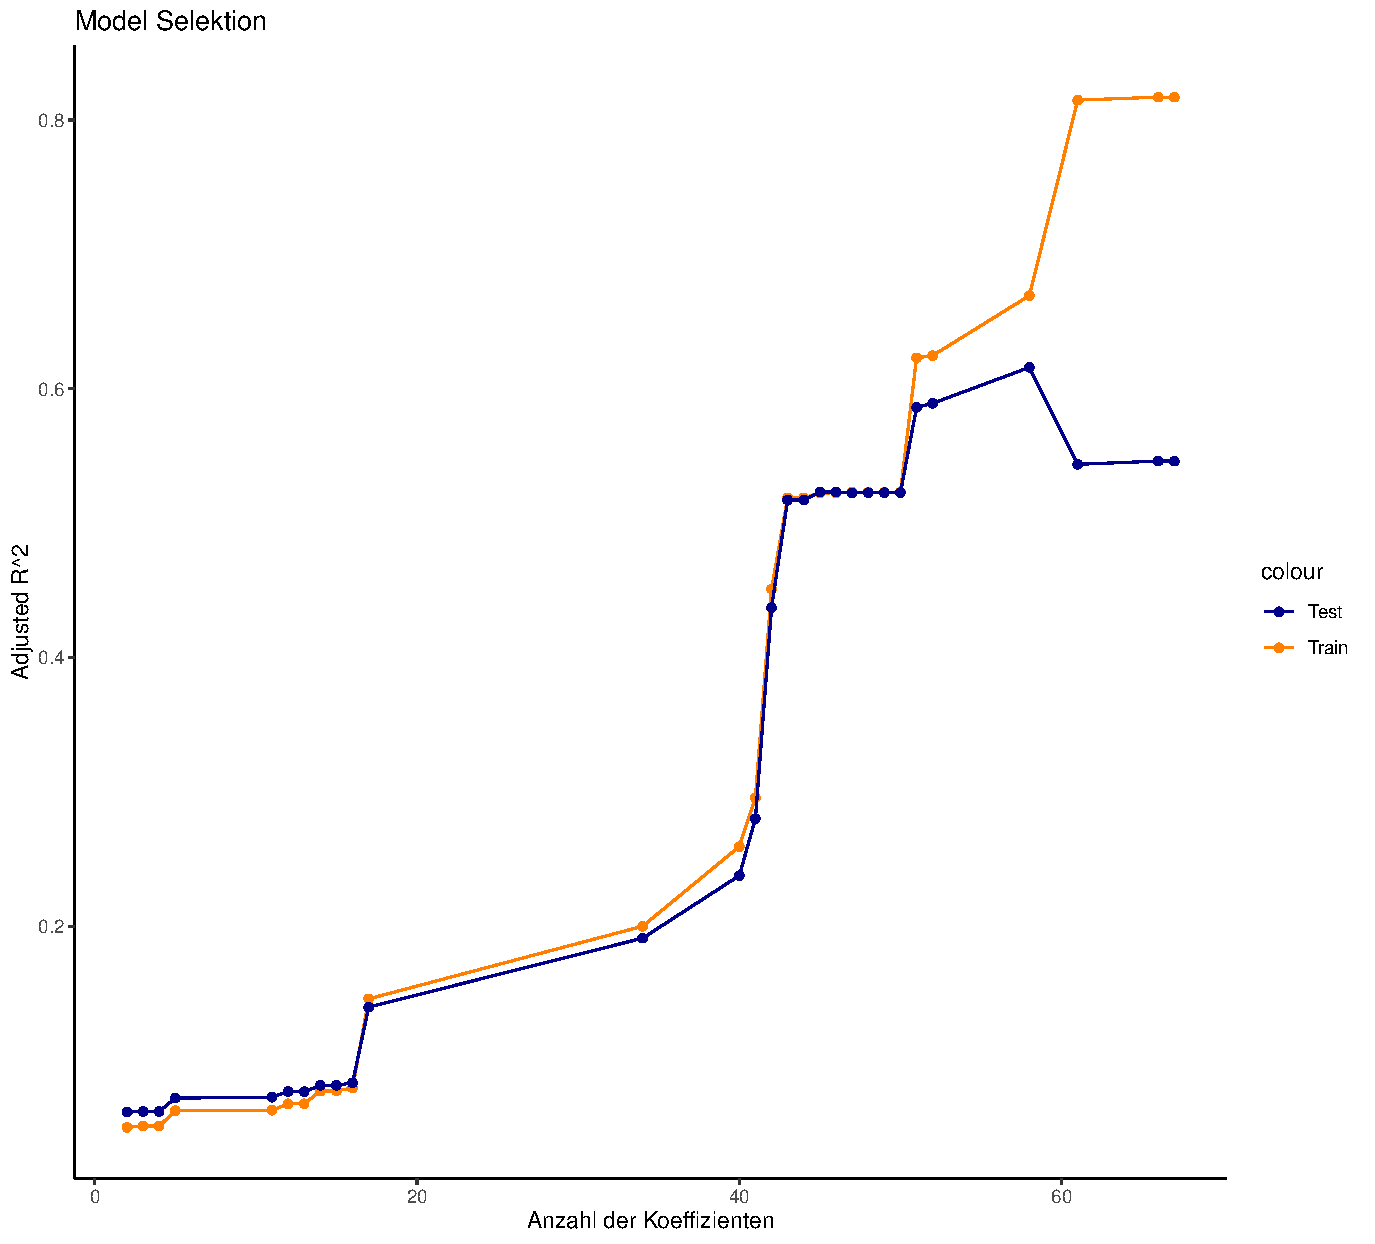
\includegraphics[width=\textwidth]{Plots/ModelSelektion1.pdf}
	\captionsource{Fahrrad Daten Mannheim und DWD}{
		Graphisches Beispiel einer Regression
	}
	\label{ModelSelektion}
\end{figure}

Auf der Y-Achse der Graphik \ref{ModelSelektion} abgetragen sehen wir die Höhe des Bestimmtheitsmaß. Auf der X Achse sehen wir die Anzahl der Koeffizienten. Mit jedem weiteren Model haben wir weitere Variablen hinzugefügt, angefangen mit den Wetter Variablen, Feiertage, Ferien, Zeitliche Variablen, wie das Jahr, Sommer oder Tageszeit bis hin zur geographischen Lage. Wir sehen, dass das Bestimmtheitsmaß, also die Genauigkeit der Vorhersage des Models, zu nimmt je mehr Variablen wir hinzufügen, bis zu einem Punkt, an dem das Bestimmtheitsmaß im Trainingsdatensatz zwar nochmals bedeutend zu nimmt, im Test Datensatz aber abnimmt. Hier geraten wir ins Overfitting. Das heißt, das Model, das hier entwickelt wurde, kann zwar die Daten, mit denen es trainiert wurde, extrem gut erklären, sobald wir aber mithilfe des Models vorhersagen treffen wollen, aufgrundlage neuer Daten, ist die Genauigkeit der Daten schlechter, als sie sein müsste. Das wollen wir verhindern. Denn wenn wir mit unserem Model Overfitting haben, kann es der Fall sein, dass wir in den Variablen Zusammenhänge sehen, die sich nicht replizieren lassen.\\

Was löst in unserem Fall das Overfitting aus? Dazu vergleichen wir den Regressions Output zweier Modelle in der Tabele \ref{ZweiModelle}. Das zweite Model ist jenes, in dem erstmals Overfitting auftritt. Das erste Model ist das Model vor diesem, in dem noch kein Overfitting auftritt.

% Table created by stargazer v.5.2.3 by Marek Hlavac, Social Policy Institute. E-mail: marek.hlavac at gmail.com
% Date and time: So, Jul 24, 2022 - 12:23:05
	
	%\scalebox{0.9}{
	\begin{longtable}{@{\extracolsep{-5pt}}lcc} 
		\caption{Log-Lineare Modele} 
		\label{ZweiModelle}
		\\[-1.8ex]\hline 
		\hline \\[-1.8ex] 
		& \multicolumn{2}{c}{\textit{Dependent variable:}} \\ 
		\cline{2-3} 
		\\[-1.8ex] & \multicolumn{2}{c}{log(Zaehlstand)} \\ 
		\\[-1.8ex] & (1) & (2)\\ 
		\hline \\[-1.8ex] 
		WertT2M & 0.027$^{***}$ & 0.027$^{***}$ \\ 
		& (0.001) & (0.001) \\ 
		WertT2M2 & 0.001$^{***}$ & 0.001$^{***}$ \\ 
		& (0.0001) & (0.0001) \\ 
		WertT2M3 & $-$0.00003$^{***}$ & $-$0.00002$^{***}$ \\ 
		& (0.00000) & (0.00000) \\ 
		WertRR & $-$0.231$^{***}$ & $-$0.229$^{***}$ \\ 
		& (0.007) & (0.005) \\ 
		WertRR2 & 0.029$^{***}$ & 0.029$^{***}$ \\ 
		& (0.001) & (0.001) \\ 
		WertRR3 & $-$0.001$^{***}$ & $-$0.001$^{***}$ \\ 
		& (0.00004) & (0.00003) \\ 
		WertF & $-$0.073$^{***}$ & $-$0.077$^{***}$ \\ 
		& (0.006) & (0.005) \\ 
		WertF2 & 0.008$^{***}$ & 0.009$^{***}$ \\ 
		& (0.002) & (0.001) \\ 
		WertF3 & $-$0.001$^{***}$ & $-$0.001$^{***}$ \\ 
		& (0.0001) & (0.0001) \\ 
		WertRF & 0.003 & 0.002 \\ 
		& (0.002) & (0.002) \\ 
		WertRF2 & $-$0.0001$^{***}$ & $-$0.0001$^{***}$ \\ 
		& (0.00003) & (0.00003) \\ 
		WertRF3 & 0.00000$^{***}$ & 0.00000$^{***}$ \\ 
		& (0.00000) & (0.00000) \\ 
		WertSD & 0.0005 & 0.0005 \\ 
		& (0.001) & (0.001) \\ 
		WertSD2 & $-$0.00000 & 0.00001 \\ 
		& (0.00004) & (0.00003) \\ 
		WertSD3 & $-$0.00000 & $-$0.00000 \\ 
		& (0.00000) & (0.00000) \\ 
		WertN & 0.010 & 0.008$^{*}$ \\ 
		& (0.006) & (0.005) \\ 
		WertN2 & $-$0.005$^{***}$ & $-$0.005$^{***}$ \\ 
		& (0.002) & (0.001) \\ 
		WertN3 & 0.0003$^{**}$ & 0.0004$^{***}$ \\ 
		& (0.0001) & (0.0001) \\ 
		FeiertagBW & $-$0.402$^{***}$ & $-$0.389$^{***}$ \\ 
		& (0.026) & (0.019) \\ 
		FeiertagRP & 0.035 & 0.043 \\ 
		& (0.162) & (0.122) \\ 
		SchulferienBW & $-$0.155$^{***}$ & $-$0.145$^{***}$ \\ 
		& (0.004) & (0.003) \\ 
		SemesterferionUM & $-$0.131$^{***}$ & $-$0.142$^{***}$ \\ 
		& (0.003) & (0.003) \\ 
		Sommer & 0.031$^{***}$ & 0.024$^{***}$ \\ 
		& (0.005) & (0.004) \\ 
		laengengrad & 3,000,977.000$^{***}$ &  \\ 
		& (14,623.910) &  \\ 
		laengengrad2 & $-$7,155.153$^{***}$ &  \\ 
		& (34.176) &  \\ 
		breitengrad & 493,372.000$^{***}$ &  \\ 
		& (2,544.529) &  \\ 
		laengenbreitengrad & $-$58,179.300$^{***}$ &  \\ 
		& (300.081) &  \\ 
		as.numeric(Jahr) & 31,617.400$^{***}$ & 2,480.775 \\ 
		& (2,353.575) & (1,764.690) \\ 
		as.numeric(Jahr2) & $-$15.658$^{***}$ & $-$1.216 \\ 
		& (1.166) & (0.874) \\ 
		as.numeric(Jahr3) & 0.003$^{***}$ & 0.0002 \\ 
		& (0.0002) & (0.0001) \\ 
		uniMA\_dist & $-$0.013$^{***}$ &  \\ 
		& (0.0001) &  \\ 
		Stunde06 & 0.404$^{***}$ & 0.404$^{***}$ \\ 
		& (0.008) & (0.006) \\ 
		Stunde07 & 0.929$^{***}$ & 0.926$^{***}$ \\ 
		& (0.008) & (0.006) \\ 
		Stunde08 & 1.078$^{***}$ & 1.072$^{***}$ \\ 
		& (0.009) & (0.006) \\ 
		Stunde09 & 0.921$^{***}$ & 0.915$^{***}$ \\ 
		& (0.009) & (0.006) \\ 
		Stunde10 & 0.817$^{***}$ & 0.811$^{***}$ \\ 
		& (0.009) & (0.007) \\ 
		Stunde11 & 0.882$^{***}$ & 0.874$^{***}$ \\ 
		& (0.009) & (0.007) \\ 
		Stunde12 & 0.997$^{***}$ & 0.990$^{***}$ \\ 
		& (0.009) & (0.007) \\ 
		Stunde13 & 1.118$^{***}$ & 1.112$^{***}$ \\ 
		& (0.009) & (0.007) \\ 
		Stunde14 & 1.172$^{***}$ & 1.165$^{***}$ \\ 
		& (0.009) & (0.007) \\ 
		Stunde15 & 1.304$^{***}$ & 1.297$^{***}$ \\ 
		& (0.009) & (0.007) \\ 
		Stunde16 & 1.466$^{***}$ & 1.458$^{***}$ \\ 
		& (0.009) & (0.007) \\ 
		Stunde17 & 1.470$^{***}$ & 1.465$^{***}$ \\ 
		& (0.009) & (0.007) \\ 
		Stunde18 & 1.283$^{***}$ & 1.281$^{***}$ \\ 
		& (0.009) & (0.006) \\ 
		Stunde19 & 1.005$^{***}$ & 1.002$^{***}$ \\ 
		& (0.009) & (0.006) \\ 
		Stunde20 & 0.698$^{***}$ & 0.698$^{***}$ \\ 
		& (0.009) & (0.006) \\ 
		Stunde21 & 0.635$^{***}$ & 0.628$^{***}$ \\ 
		& (0.050) & (0.037) \\ 
		Stunde22 & 0.548$^{***}$ & 0.534$^{***}$ \\ 
		& (0.049) & (0.037) \\ 
		WochentagDo & $-$0.007 & $-$0.005 \\ 
		& (0.006) & (0.004) \\ 
		WochentagFr & $-$0.084$^{***}$ & $-$0.083$^{***}$ \\ 
		& (0.006) & (0.004) \\ 
		WochentagMi & $-$0.001 & $-$0.002 \\ 
		& (0.006) & (0.004) \\ 
		WochentagMo & $-$0.050$^{***}$ & $-$0.046$^{***}$ \\ 
		& (0.006) & (0.004) \\ 
		WochentagSa & $-$0.626$^{***}$ & $-$0.626$^{***}$ \\ 
		& (0.006) & (0.004) \\ 
		WochentagSo & $-$0.970$^{***}$ & $-$0.968$^{***}$ \\ 
		& (0.006) & (0.004) \\ 
		Adenauer-Brücke &  & 0.185$^{***}$ \\ 
		&  & (0.004) \\ 
		Kurpfalzbrücke &  & 1.549$^{***}$ \\ 
		&  & (0.004) \\ 
		K-Schumacher-Brücke &  & $-$2.609$^{***}$ \\ 
		&  & (0.004) \\ 
		Lindenhofüberführung &  & $-$0.507$^{***}$ \\ 
		&  & (0.005) \\ 
		Neckarauer Übergang &  & $-$0.039$^{***}$ \\ 
		&  & (0.005) \\ 
		Renzstraße &  & 0.861$^{***}$ \\ 
		&  & (0.004) \\ 
		Schlosspark Lindenhof &  & 0.180$^{***}$ \\ 
		&  & (0.005) \\ 
		FeiertagBW:FeiertagRP & $-$0.519$^{***}$ & $-$0.535$^{***}$ \\ 
		& (0.164) & (0.123) \\ 
		Constant & $-$46,216,015.000$^{***}$ & $-$1,687,396.000 \\ 
		& (1,582,933.000) & (1,187,073.000) \\ 
		\hline \\[-1.8ex] 
		Observations & 328,715 & 328,715 \\ 
		R$^{2}$ & 0.668 & 0.814 \\ 
		Adjusted R$^{2}$ & 0.668 & 0.814 \\ 
		Residual Std. Error & 0.842 (df = 328659) & 0.631 (df = 328657) \\ 
		F Statistic & 12,043.5$^{***}$  & 25,194.4$^{***}$ \\ 
		&(df = 55; 328659)& (df = 57; 328657)\\
		\hline 
		\hline \\[-1.8ex] 
		\textit{Note:}  & \multicolumn{2}{r}{$^{*}$p$<$0.1; $^{**}$p$<$0.05; $^{***}$p$<$0.01} \\ 
	\end{longtable}
	%}

Beide Modelle unterscheiden sich im wesentlichen in der Wahl der Fixed Effects. Fixed Effects sind all jene Schätzer, die über die Zeit nicht variieren, also fix sind und nur zwischen den Entitäten variieren. In diesem konkreten Fall heißt das, ein Fixed Effect ist eine Variable die zeitlich konstant bleibt, sich aber zwischen den Fahrradzählstationen unterscheidet. Das dient dazu, die Unterschiede zwischen diesen Stationen zu messen und im Model mit aufzunehmen. Denn wenn wir uns die Graphik \ref{BoxplotStationen} anschauen, sehen wir, dass die Stationen untereinander recht stark variieren. Z.B. sehen wir, dass auf der Kurpfalzbrücke, die von der Innenstadt über den Neckar führt, grundsätzlich mehr Radverkehr herrscht. Nehmen wir jetzt z.B. eine Dummy Variable in das Model auf, die 1 ist, wenn ein Beobachtungswert von der Kurpfalzbrücke stammte und 0 ist, wenn der Beobachtungswert von einer anderen Station stammte, dann erklärt diese Variable den Unterschied zwischen der Kurpfalzbrücke und den anderen Stationen im Model, ohne den Ursächlichen Grund dafür zu kennen, erhöht aber den Fit des Models, denn nun können die anderen Variablen ihren Einfluss präziser schätzen.\\ 

Eine solche Dummy Variable können wir für 7 von 8 Stationen in das Model aufnehmen. Bei der achten reicht es, wenn alle anderen Dummy Variablen 0 sind. Andernfalls bekämen wir ein multikollineares Model, also ein Model in dem mindestens zwei Variablen linear abhängig von einander sind. Genau auf diese Weise sind wir im zweiten Model vorgegangen. Dieses beinhaltet eine Dummy Variable Kurpfalzbrücke, Lindenhofüberführung, Neckarauer Übergang, Renzstraße und Schloßpark/Lindenhof. Die übrige Station an der Kurt Schuhmacher Brücke ergibt sich, wie bereits erklärt, wenn alle anderen 7 Dummy Variabeln 0 sind. Diese Vorgehensweise fürht zu einem Bestimmtheitsmaß von 81,44 \%, was sich gut anhört, wie aber bereits gezeigt, größtenteils auf Overfitting zurückzuführen ist.\\

Möglicherweise hängt dies damit zu zusammen, dass die Stations Dummy Variabeln zwar Unterschiede erkennen, aber keinen ursächlichen Grund dafür finden. Wenn man aber Lageparameter als Fixed Effekt nutzt hätte man einen möglichen ursächlichen Grund für den Unterschied, die Lage. Da Lageparameter zeitlich auch konstant sind, lassen sich diese ebenfalls sehr gut als Fixed Effect nutzen. Im ersten Model nutzen wir dazu den Längengrad, sowie den quadrierten Längengrad, den Breitengrad, Längen und Breitengrad miteinander multipliziert (Intersektion) und den Abstand zur Universität Mannheim in uniMA dist. Auf den quadrierten Wert des Breitengrades verzichten wir, weil dies wiederum zu Multikollinearität führen würde und im Regressionsoutput ein Fehler auftauchen würde, wie sich zeigte. Auch führt eine Kombination aus Lageparametern und Standort Dummy Variabeln zu Fehlern im Regressionsoutput, weswegen wir beide Fixed Effects getrennt von einander nutzen.\\

Obwohl wir bei dem Model mit den Lageparametern ein kleineres Bestimmtheitsmaß von nur 66,8 \% erhalten, entscheiden wir uns gegen das Model mit Standort Dummy Variabeln, wegen einer höheren externen Validität gemessen im Test Datensatz.

\chapter{Fazit}

\chapter{Anhang}

\begin{figure}[!ht]
	\centering
	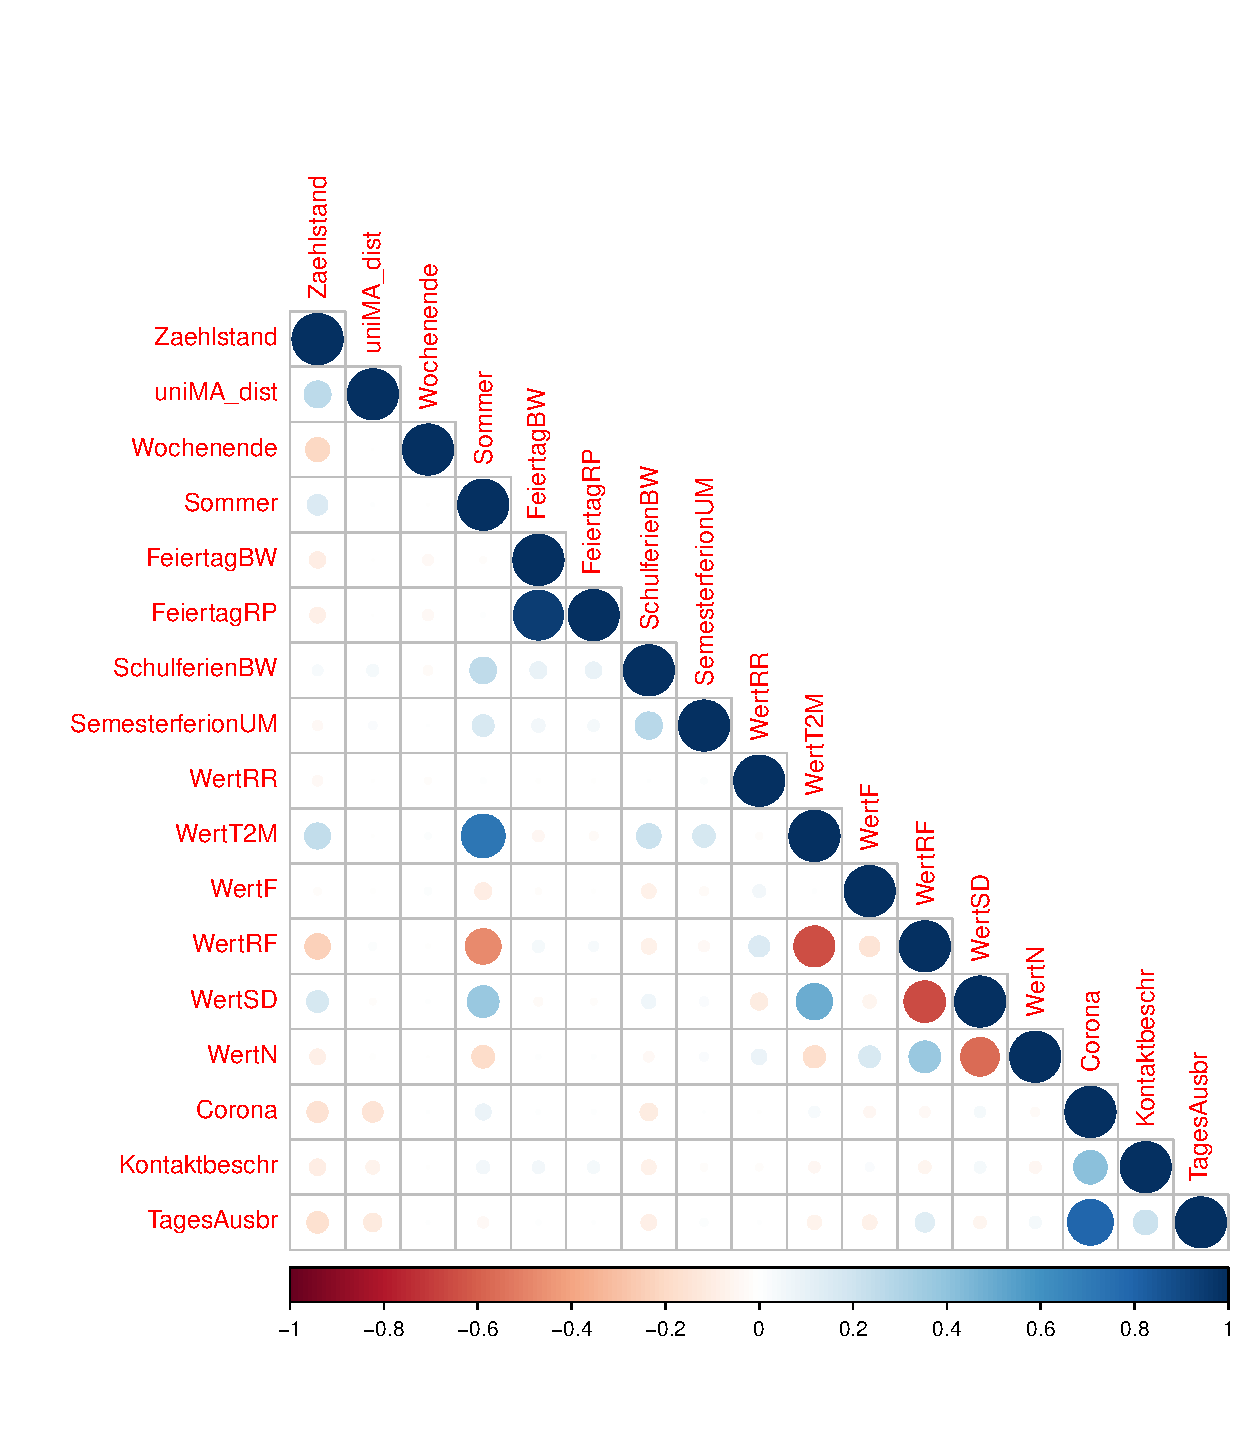
\includegraphics[width=\textwidth]{Plots/Corr_Plot.pdf}
	\captionsource{Korrelations Plot}{
		Korrelation zwischen den verschiedenen Variablen
	}
	\label{fig:meine-grafik5}
\end{figure}

\begin{figure}[!ht]
	\centering
	\includegraphics[width=\textwidth]{Plots/Monatliche_Temperatur_Niederschläge.png}
	\captionsource{Monatliche Durchschnittliche Temperaturen und maximale Niederschläge nach Tageszeiten in 2018}{
		DWD, eigene Darstellung
	}
	\label{fig:meine-grafik5}
\end{figure}

\begin{figure}[!ht]
	\centering
	\includegraphics[width=\textwidth]{Plots/Taegliche_Temperatur_Niederschläge.png}
	\captionsource{Tägliche Durchschnitts Temperaturen und monatliche maximale Niederschläge nach Tageszeiten in 2018}{
		DWD, eigene Darstellung
	}
	\label{fig:meine-grafik5}
\end{figure}

\begin{table}[!htbp] \centering 
	\caption{Freizeit und Berufsverkehr im Vergleich} 
	\label{utilitarianvsFreizeit} 
	\begin{tabular}{@{\extracolsep{-5pt}}lccccc} 
		\\[-1.8ex]\hline 
		\hline \\[-1.8ex] 
		%\\[-1.8ex] & \multicolumn{8}{c}{log(Zaehlstand)}  \\ 
		\\[-1.8ex] & Freizeit & & & Utilitarist. & \\ 
		\hline \\[-1.8ex] 
		
		Leichter Nieselregen & -0.208830$^{***}$ & (0.025861) & $<$ & -0.063944$^{***}$ & (0.013529)\\ 
		
		Starker Nieselregen & -0.242996$^{***}$ & (0.044008) & $<$ & -0.071652$^{**}$ & (0.023158)\\ 
		
		Leichter Regen & -0.350410$^{***}$ & (0.051344) & $<$ & -0.125781$^{***}$ & (0.025659)\\ 
		
		Moderater Regen & -0.318279$^{***}$ & (0.070454) & $<$ & -0.120595$^{**}$ & (0.037419)\\ 
		
		Starker Regen & -0.269545$^{*}$ & (0.127235) & $<$ & -0.128016 & (0.073305)\\ 
		
		Heftiger Regen & -0.055661 & (0.205122) & $>$ & -0.106119 & (0.137777)\\ 
		
		Temperatur & 0.050447$^{***}$ & (0.002065) & $>$ & 0.011108$^{***}$ & (0.001199)\\ 
		
		Temperatur$^2$ & -0.000884$^{***}$ & (0.000061) & $<$ & -0.000151$^{***}$ & (0.000040)\\ 
		
		Wind & -0.034832$^{***}$ & (0.003017) & $<$ & -0.012150$^{***}$ & (0.001781)\\ 
		
		rel. Feuchte & -0.002215$^{***}$ & (0.000390) & $<$ & -0.000288 & (0.000243)\\ 
		
		Sonne & -0.000013 & (0.000284) & $>$ & -0.000184 & (0.000183)\\ 
		
		Bedeckung & -0.007426$^{***}$ & (0.001721) & $<$ & -0.002814$^{*}$ & (0.001122)\\ 
		
		FeiertagBW & -0.140294 & (0.111894) & $>$ & -0.207367$^{***}$ & (0.053588)\\ 
		
		FeiertagRP & -0.369612$^{**}$ & (0.115990) & $<$ & -0.085082 & (0.056197)\\ 
		
		SchulferienBW & -0.065830$^{***}$ & (0.010924) & $<$ & -0.065506$^{***}$ & (0.007072)\\ 
		
		SemesterferienUM & -0.068875$^{***}$ & (0.010248) & $<$ & -0.028236$^{***}$ & (0.006324)\\ 
		
		Sommer & 0.076692$^{***}$ & (0.014095) & $>$ & 0.029047$^{***}$ & (0.008655)\\ 
		
		Kontaktbeschr & -0.084528$^{***}$ & (0.014799) & $<$ & -0.036209$^{***}$ & (0.008175)\\ 
		
		Observations & 44,649 & & & 37,438 & \\ 
		Adjusted psydo R$^{2}$ & 0.093052 & & & 0.041806 & \\  
		\hline \\[-1.8ex] 
		\textit{Fixed Effects:} & \multicolumn{5}{l}{Standort: 8;Stunde: 18;Wochentag: 7;Jahr: 9} \\ 
		\textit{Notes:} & \multicolumn{5}{l}{$^{***}$Significant at the 1 percent level.} \\ 
		& \multicolumn{5}{l}{$^{**}$Significant at the 5 percent level.} \\ 
		& \multicolumn{5}{l}{$^{*}$Significant at the 10 percent level.} \\ 
	\end{tabular} 
\end{table} 






\begin{table}[!htbp] \centering 
	\caption{Wetterdaten als täglichen Niederschlag und Höchsttemperatur} 
	\label{utilitarianvsFreizeit} 
	\begin{tabular}{@{\extracolsep{-5pt}}lccccc} 
		\\[-1.8ex]\hline 
		\hline \\[-1.8ex] 
		%\\[-1.8ex] & \multicolumn{8}{c}{log(Zaehlstand)}  \\ 
		\\[-1.8ex] & Standardmodell & & & taeglWetter & \\ 
		\hline \\[-1.8ex] 
		
		Leichter Nieselregen & -0.183609$^{***}$ & (0.015146) &  &  & \\ 
		
		Starker Nieselregen & -0.248702$^{***}$ & (0.012068) &  &  & \\ 
		
		Leichter Regen & -0.331162$^{***}$ & (0.020894) &  &  & \\ 
		
		Moderater Regen & -0.353010$^{***}$ & (0.018780) &  &  & \\ 
		
		Starker Regen & -0.373162$^{***}$ & (0.043303) &  &  & \\ 
		
		Heftiger Regen & -0.208576$^{**}$ & (0.051431) &  &  & \\ 
		
		Täglicher Regen &  &  &  & -0.001410$^{***}$ & (0.000094)\\ 
		
		Temperatur & 0.036044$^{***}$ & (0.004718) & & \\ 
		
		Temperatur$^2$ & -0.000482$^{***}$ & (0.000052) &  &  & \\ 
		
		TagesHöcshttemp & &  &  & 0.034072$^{***}$ & (0.005517)\\ 
		
		TagesHöcshttemp$^2$ &  &  &  & -0.000353$^{**}$ & (0.000081)\\ 
		
		Wind & -0.040923$^{***}$ & (0.002549) & $<$ & -0.035015$^{***}$ & (0.002136)\\ 
		
		rel. Feuchte & -0.003787$^{**}$ & (0.001078) & $>$ & -0.004337$^{**}$ & (0.000948)\\ 
		
		Sonne & -0.000118 & (0.000086) & $>$ & 0.000179 & (0.000115)\\ 
		
		Bedeckung & -0.008657$^{***}$ & (0.001074) & $<$ & -0.000208 & (0.000694)\\ 
		
		FeiertagBW & -0.459770$^{***}$ & (0.080732) & $<$ & -0.444115$^{**}$ & (0.085660)\\ 
		
		FeiertagRP & -0.414345$^{***}$ & (0.059184) & $>$ & -0.427126$^{***}$ & (0.065291)\\ 
		
		SchulferienBW & -0.138772$^{***}$ & (0.020264) & $<$ & -0.138865$^{***}$ & (0.020478)\\ 
		
		SemesterferienUM & -0.159223$^{**}$ & (0.030637) & $<$ & -0.150810$^{**}$ & (0.036192)\\ 
		
		Sommer & 0.082386$^{**}$ & (0.020602) & $>$ & 0.072395$^{*}$ & (0.022105)\\ 
		
		Kontaktbeschr & -0.133188$^{**}$ & (0.026552) & $>$ & -0.139072$^{**}$ & (0.026333)\\ 
		
		Observations & 410,891 & & & 410,891 & \\ 
		Adjusted R$^{2}$ & 0.817542 & & & 0.817554 & \\  
		\hline \\[-1.8ex] 
		\textit{Fixed Effects:} & \multicolumn{5}{l}{Standort: 8;Stunde: 18;Wochentag: 7;Jahr: 9} \\ 
		\textit{Notes:} & \multicolumn{5}{l}{$^{***}$Significant at the 1 percent level.} \\ 
		& \multicolumn{5}{l}{$^{**}$Significant at the 5 percent level.} \\ 
		& \multicolumn{5}{l}{$^{*}$Significant at the 10 percent level.} \\ 
	\end{tabular} 
\end{table} 

Zwar steigt das Bestimmtheitsmaß und die Übersichtlichkeit des Modells nimmt zu, da die Anzahl der Koeffizienten abnimmt, allerdings verwirrt es mich, dass Feiertage in Badenwürttemberg eine niedrigere Signifikanz haben sollen, als in Rheinlandpfalz. Auch dass die Sommer Variable an Signifikanz weiter verliert, macht mich eher skeptisch.



\newpage
\addcontentsline{toc}{chapter}{Literaturverzeichnis}
\bibliography{bib1}

\end{document}

